\chapter{Σύγχρονοι Υπερβαθμωτοί Επεξεργαστές}
\label{chap2}

\section{Εισαγωγή}
\label{chap2_Intro}

Οι υπερβαθμωτοί επεξεργαστές \cite{nikolos2012architecture} αποτελούν ένα πολύ σημαντικό επίτευγμα σχεδίασης στην αρχιτεκτονική υπολογιστών καθώς προσέφεραν τη δυνατότητα παραλληλισμού σε επίπεδο εντολών. Συνεπώς, με τη χρήση ενός και μόνο επεξεργαστή επιτυγχάνεται η εκτέλεση πολλαπλών εντολών ταυτόχρονα, οδηγώντας σε ταχύτερη ολοκλήρωση υπολογισμών. Με την πάροδο των ετών από την πρώιμη εποχή των υπερβαθμωτών επεξεργαστών πληθώρα τεχνικών έχουν αναπτυχθεί για τη μείωση της κατανάλωσης ενέργειας σε αυτούς, δίνοντας έτσι τη δυνατότητα ενσωμάτωσής τους σε όλα σχεδόν τα τεχνολογικά προϊόντα.

%----------------------------------------------------------%

\section{Ιστορική Αναδρομή}
\label{chap2_History}

Η ανάπτυξη των υπερβαθμωτών επεξεργαστών και η επικράτησή τους έναντι των προγόνων του αποτέλεσε καθοριστικό παράγοντα στην ραγδαία αύξηση της απόδοσης των επεξεργαστών. Η εμφάνιση του πρώτου υπερβαθμωτού επεξεργαστή στην αγορά το 1993, ο αποκαλούμενος \en{Pentium P5} της \en{Intel} \cite{saini1993design}, έπαιξε καθοριστικό ρόλο στην επικράτηση του σχεδιαστή στην αγορά των μικροεπεξεργαστών.
\par
Πρόγονο του υπερβαθμωτού επεξεργαστή αποτέλεσαν οι βαθμωτοί επεξεργαστές, οι οποίοι εισήγαγαν την τεχνική των μερικώς επικαλυπτόμενων λειτουργιών. Σύμφωνα με την τεχνική αυτή, η μονάδα επεξεργασίας χωρίζεται σε βαθμίδες όπου κάθε βαθμίδα εκτελεί μια ξεχωριστή λειτουργία με δυνατότητα εξυπηρέτησης μιας εντολής ανά κύκλο. Παρόλο που ο συνολικός χρόνος μιας εντολής από την προσκόμισή της στον επεξεργαστή έως την ολοκλήρωσή της παραμένει ίδιος, ο συνολικός απαιτούμενος χρόνος  πολλαπλών εντολών μειώνεται καθώς επιτυγχάνεται η ολοκλήρωση μιας εντολής ανά κύκλο ρολογιού.
\par
Η αύξηση της απόδοσης ενός επεξεργαστεί ισοδυναμεί με τη μείωση του συνολικού χρόνου εκτέλεσης των προγραμμάτων σε αυτόν, συνεπώς την αύξηση του αριθμού εντολών που ολοκληρώνονται σε κάθε κύκλο (ρυθμός ολοκλήρωσης εντολών). Η απλή εφαρμογή της τεχνικής μερικώς επικαλυπτόμενων λειτουργιών, των βαθμωτών επεξεργαστών, δεν επαρκούσε για την περαιτέρω βελτίωσή του ρυθμού ολοκλήρωσης. Τη λύση έδωσε η σχεδίαση των υπερβαθμωτών επεξεργαστών οι οποίοι αποτελούνται από παράλληλες μονάδες μερικώς επικαλυπτόμενων λειτουργιών, διαφοροποιημένες κατάλληλα ώστε να παρέχουν πολλαπλές και ξεχωριστές λειτουργίες, παρέχοντας έτσι το πλεονέκτημα της παράλληλης εκτέλεσης εντολών. Στη βιβλιογραφία, το πλήθος των παράλληλων μονάδων μερικώς επικαλυπτόμενων λειτουργιών αποκαλείται και πλάτος του υπερβαθμωτού επεξεργαστή ή βαθμός παραλληλίας.
\par
Οι υπερβαθμωτοί επεξεργαστές που αναπτύχθηκαν χωρίζονται σε δύο βασικές κατηγορίες, τους στατικούς που εκτελούν τις εντολές με τη σειρά που βρίσκονται στο πρόγραμμα, και τους δυναμικούς που έχουν τη δυνατότητα να εκτελούν τις εντολές με διαφορετική σειρά από αυτή του αρχικού προγράμματος. Παρόλο που στην περίπτωση του δυναμικού επεξεργαστή η σειρά εκτέλεση των εντολών μεταβάλλεται, το τελικό αποτέλεσμα τους δεν αλλοιώνεται καθώς ο επεξεργαστής είναι αρμόδιος ώστε οι εντολές να ολοκληρώνονται με τη σωστή σειρά. Η βελτίωση της απόδοσης που προσέφερε η εκτός-σειράς εκτέλεση, οδήγησε στην επικράτησή τους έναντι των στατικών. Αυτό είναι και ο λόγος για τον οποίο η παρούσα μελέτη επικεντρώνεται στη συγκεκριμένη κατηγορία, στην οποία ανήκουν και οι εμπορικοί υπερβαθμωτοί επεξεργαστές.

%----------------------------------------------------------%

\begin{figure}[!h]
    \centering
    \fbox{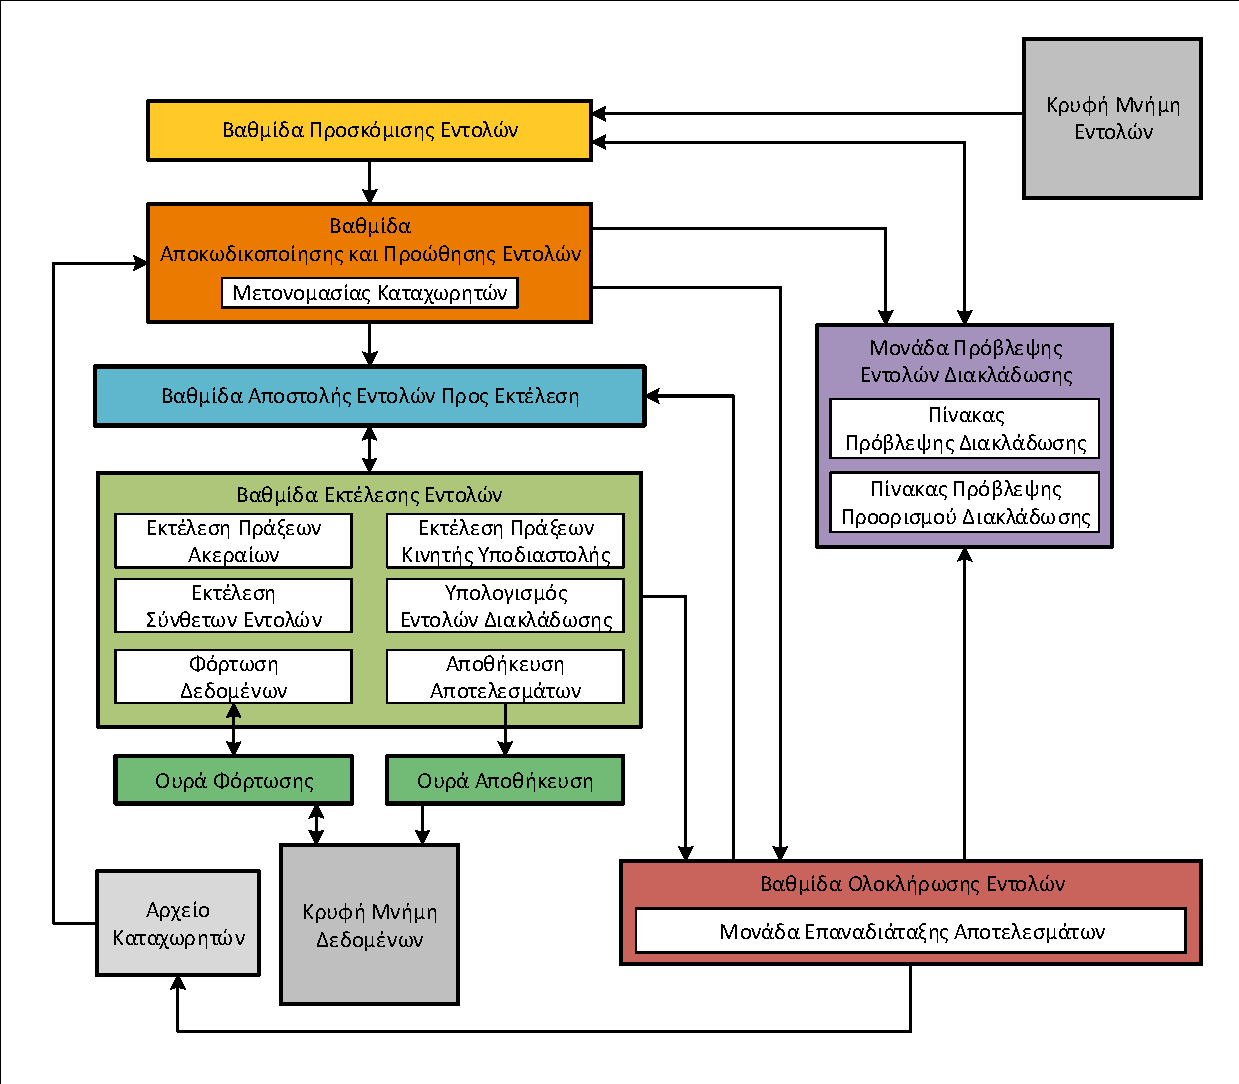
\includegraphics[width=0.95\linewidth, trim=0.5cm 0.8cm 0.5cm 0.5cm, clip=true]{\hardwareDIR/chap2_pipeline_stages.pdf}}
    \caption{Δομή Μηχανισμού Μερικώς Επικαλυπτόμενων Λειτουργιών}
    \label{fig:chap2_pipeline_stages}
\end{figure}

\section{Δομή και Οργάνωση του Δυναμικού Υπερβαθμωτού Επεξεργαστή}
\label{chap2_Superscalar}

Παρότι η δομή των υπερβαθμωτών επεξεργαστών εμφανίζει πλέον πολλές διαφοροποιήσεις μεταξύ σχεδιαστών και γενεών, οι μονάδες που τους αποτελούν μπορούν να διαχωριστούν σε πέντε βαθμίδες, όπως παρουσιάζονται στο Σχήμα \ref{fig:chap2_pipeline_stages}.

\subsubsection*{Προσκόμιση Εντολών}
\label{chap2_InstructionFetchUnit}

Στην πρώτη βαθμίδα ενός υπερβαθμωτού επεξεργαστή υλοποιείται ο μηχανισμός προσκόμιση εντολών από την Κρυφή Μνήμη Εντολών πρώτου επιπέδου. Σε κάθε κύκλο μπορούν να προσκομιστούν ένα σύνολο εντολών, το μέγιστο πλήθος των οποίων καθορίζεται από το πλάτος του υπερβαθμωτού επεξεργαστή.
\par
Για την απρόσκοπτη λειτουργία του μηχανισμού σε κάθε κύκλο πρέπει να είναι διαθέσιμες τόσες εντολές όσες και ο μέγιστος αριθμός εντολών που μπορούν να αποκωδικοποιηθούν ταυτόχρονα, διαδικασία η οποία εκτελείται στην αμέσως επόμενη βαθμίδα. Για το λόγο αυτό εισάγεται μια προσωρινή μνήμη εντολών στο τέλος της βαθμίδας προσκόμισης εντολών, στην οποία αποθηκεύονται οι εντολές που έχουν προσκομιστεί έως ότου προωθηθούν στη βαθμίδα αποκωδικοποίησης.
\par
Τέλος, προτού γίνει η προσκόμιση νέων εντολών στη βαθμίδα, προηγείται ο υπολογισμός της διεύθυνσης Κρυφής Μνήμης Εντολών στην οποία είναι αποθηκευμένες. Για το σκοπό αυτό, στη βαθμίδα προσκόμισης εντολών εμπεριέχονται και δυο ακόμα βασικά στοιχεία, η Μονάδα Υπολογισμού Διεύθυνσης της αμέσως επόμενης εντολής και η Μονάδα Δυναμικής Πρόβλεψης Διακλαδώσεων. Η Μονάδα Δυναμικής Πρόβλεψης Διακλαδώσεων αποτελεί τον κορμό της παρούσας διπλωματικής, επομένως η αναλυτική περιγραφή της λειτουργίας της πραγματοποιείται ξεχωριστά στην Ενότητα \ref{chap2_DynamicBranchPredictionUnit}.

\subsubsection*{Αποκωδικοποίηση και Προώθηση Εντολών}
\label{chap2_InstructionDecodeDispatch}

Βασική λειτουργία της δεύτερης βαθμίδα του υπερβαθμωτού επεξεργαστή είναι η αποκωδικοποίηση των εντολών χαμηλού επιπέδου σε μικροεντολές. Στη συνέχεια πραγματοποιείται ο έλεγχος εξαρτήσεων μεταξύ των εντολών καθώς και η προσκόμιση των τιμών των τελουμένων από το αρχείο καταχωρητών.
\par
Εξαιτίας της μεταβαλλόμενης σειράς εκτέλεσης των εντολών, μεταξύ των εντολών εμφανίζονται εξαρτήσεις δεδομένων οι οποίες καθιστούν αδύνατη την εκτέλεσή τους σε διαφορετική σειρά. Τα είδη των εξαρτήσεων δεδομένων εντάσσονται σε τρεις κατηγορίες:\\
\textit{Ανάγνωσης μετά από Εγγραφή (ΑμΕ) -} Όταν η Εντολή Β που μόλις αποκωδικοποιήθηκε αναμένει το αποτέλεσμα της προηγούμενης Εντολής Α, το οποίο χρησιμοποιείται ως τελούμενο από την Εντολή Β (καταχωρητής προορισμού Α = καταχωρητή πηγής Β).\\
\textit{Εγγραφή μετά από Εγγραφή (ΕμΕ) -} Όταν η Εντολή Β που μόλις αποκωδικοποιήθηκε αναμένει την εκτέλεση της προηγούμενης Εντολής Α, διότι και οι δύο αποθηκεύουν το αποτέλεσμά τους στον ίδιο καταχωρητή (καταχωρητής προορισμού Α = καταχωρητή προορισμού Β).\\
\textit{Εγγραφής μετά από Ανάγνωση (ΕμΑ) -} Όταν η Εντολή Β που μόλις αποκωδικοποιήθηκε αναμένει την εκτέλεση της προηγούμενης Εντολής Α, διότι η Εντολή Β αποθηκεύει τιμή στον ίδιο καταχωρητή από τον οποίο πραγματοποιεί ανάγνωση η εντολή Α (καταχωρητής πηγής Α = καταχωρητή προορισμού Β).
\par
Και οι τρεις αυτές περιπτώσεις εξαρτήσεων επιβάλουν την αδυναμία εκτέλεσης ορισμένων εντολών (Εντολή Β) έως ότου οι εξαρτήσεις παύσουν να ισχύουν, συνεπώς έως ότου εκτελεστούν οι προηγούμενες εντολές που αλληλεπιδρούν σε κοινούς καταχωρητές (Εντολή Α). Η συνεχής εμφάνιση εξαρτήσεων μπορεί να οδηγήσει σε σημαντική υποβάθμιση της απόδοσης του συστήματος. Από τα τρία είδη εξαρτήσεων που παρουσιάστηκαν, οι εξαρτήσεις τύπου ΕμΕ και ΕμΑ θα ήταν δυνατό να αποφευχθούν μέσω της χρήσης μεγαλύτερου πλήθους καταχωρητών από τις μικροεντολές. Οι εξαρτήσεις τέτοιου είδους αποκαλούνται αντεξαρτήσεις. Στους σύγχρονους υπερβαθμωτούς επεξεργαστές εισάγεται μία επιπλέον λειτουργία στη βαθμίδα αυτή η οποία αναλαμβάνει την επίλυση των αντεξαρτήσεων μέσω της αντιστοίχησης των αρχιτεκτονικών καταχωρητών, που χρησιμοποιούνται από τις εντολές χαμηλού επιπέδου, σε ένα μεγαλύτερο σύνολο φυσικών καταχωρητών που βρίσκονται εντός του Μηχανισμού Μερικώς Επικαλυπτόμενων Λειτουργιών. Η διαδικασία αυ΄τη αποκαλείται Μετονομασία Καταχωρητών και σε πολλές περιπτώσεις επεξεργαστών αποτελεί ξεχωριστή βαθμίδα.
\par
Μόλις ολοκληρωθεί και η μετονομασία των καταχωρητών μίας εντολής, αυτή προωθείται στην επόμενη βαθμίδα όπου αναμένει έως ότου όλα τα τελούμενα της είναι διαθέσιμα. Επιπλέον, η εντολή καταλαμβάνει μία θέση στη Μονάδα Επαναδιάταξης Αποτελεσμάτων, όπου συγκεντρώνονται τα αποτελέσματα των εντολών ώστε η ολοκλήρωσή τους να γίνεται με τη σωστή σειρά.

\subsubsection*{Αποστολή Εντολών Προς Εκτέλεση}
\label{chap2_InstructionIssue}

Οι εντολές που έχουν αποκωδικοποιηθεί και μετονομαστεί αποθηκεύονται σε μία προσωρινή μνήμη έως ότου είναι διαθέσιμα όλα τα τελούμενα που χρησιμοποιούν. Στου σύγχρονους υπερβαθμωτούς επεξεργαστές κάθε λειτουργική μονάδα έχει τη δική της προσωρινή μνήμη ώστε να διαχωρίζονται οι εντολές που αποστέλλονται από την προηγούμενη βαθμίδα. Οι μνήμες αυτές αποκαλούνται συνήθως Σταθμοί Κράτησης καθώς αποθηκεύονται τα τελούμενα που απαιτούνται από την εντολή, έως την εκτέλεση της. Μόλις όλα τα τελούμενα είναι διαθέσιμα και η αντίστοιχη λειτουργική μονάδα ελευθερωθεί πραγματοποιείται η προώθηση των τελουμένων της εντολής ώστε να πραγματοποιηθεί η εκτέλεσή της. Με το πέρας της εκτέλεσης γίνεται και η ενημέρωση όλων των Σταθμών Κράτησης που αναμένουν το αποτέλεσμα της συγκεκριμένης εντολής (εξαρτήσεις δεδομένων τύπου ΑμΕ).

\subsubsection*{Εκτέλεση Εντολών}
\label{chap2_InstructionExcecution}

Οι σύγχρονοι υπερβαθμωτοί επεξεργαστές αποτελούνται από ένα πλήθος διαφορετικών λειτουργικών μονάδων ώστε η κάθε μία να είναι βελτιστοποιημένη σε ένα συγκεκριμένο είδος πράξεων, με ορισμένες από αυτές να διαθέτουν τη δυνατότητα εκτέλεσης πολλαπλών εντολών στον ίδιο κύκλο ρολογιού. Στις πρώιμες εκδοχές των υπερβαθμωτών επεξεργαστών η μονάδα εκτέλεσης χρησιμοποιούταν τόσο για την εκτέλεση αριθμητικών πράξεων όσο για τον υπολογισμό διευθύνσεων μνήμης, την εκτέλεση εντολών διακλάδωσης, τη φόρτωση δεδομένων από την κρυφή μνήμη και την αποθήκευση αποτελεσμάτων σε αυτή. Πλέον συνηθίζεται οι λειτουργίες αυτές να υλοποιούνται από ξεχωριστές μονάδες. Η Μονάδα Υπολογισμού Διεύθυνσης υπολογίζει τη νέα τιμή του μετρητή προγράμματος, η οποία στην περίπτωση εντολών διακλάδωσης συγκρίνεται με την προβλεπόμενη διεύθυνση προσκόμισης. Αντίστοιχα, η Μονάδα Φόρτωσης/Αποθήκευσης συνδέεται απευθείας με την Κρυφή Μνήμη Δεδομένων για άμεση διαχείριση των δεδομένων από και προς αυτή.
\par
Ώς βαθμός παραλληλίας ορίζεται ο μέγιστος αριθμός εντολών που μπορούν να προσκομιστούν, να αποκωδικοποιηθούν ή να ολοκληρωθούν σε κάθε κύκλο. Στις πρώτες βαθμίδες ο χρόνος που απαιτείται σε κάθε μία δεν είναι σταθερός μεταξύ των διαφορετικών εντολών. Αντίθετα, στο στάδιο της εκτέλεσης ο χρόνος είναι σταθερός καθώς τα δεδομένα είναι όλα διαθέσιμα και πλέον αρκεί η εκτέλεση της απαιτούμενης ενέργειας. Για να μην εισάγεται καθυστέρηση στο στάδιο αυτό λόγω έλλειψης πόρων (δομικές εξαρτήσεις) ο συνολικός αριθμός λειτουργικών μονάδων πρέπει να υπερβαίνει το βαθμό παραλληλίας.
\par
Με το πέρας της εκτέλεσης γίνεται και η ενημέρωση όλων των Σταθμών Κράτησης που αναμένουν το αποτέλεσμα της συγκεκριμένης εντολής. Εξαιτίας της εκτέλεσης των εντολών με διαφορετική σειρά από αυτή του αρχικού προγράμματος, τα αποτελέσματα που εξάγεται από τις λειτουργικές μονάδες δεν επιτρέπεται να αποθηκευτούν στον αντίστοιχο αρχιτεκτονικό καταχωρητή έως ότου εκτελεστούν όλες οι εντολές που προηγούνται. Για το λόγο αυτό τα αποτελέσματα προωθούνται στην αντίστοιχη θέση που καταλαμβάνει η εντολή στη Μονάδα Επαναδιάταξης Αποτελεσμάτων, η οποία εντάσσεται στην αμέσως επόμενη βαθμίδα.

\subsubsection*{Ολοκλήρωση Εντολών}
\label{chap2_InstructionCommit}

Όταν μια εντολή περάσει όλες τις προηγούμενες βαθμίδες και το αποτέλεσμά της είναι διαθέσιμο στην έξοδο της λειτουργικής μονάδας, δεν μπορεί να θεωρηθεί ότι ολοκληρώθηκε διότι η σειρά ολοκλήρωσης των εντολών πρέπει να είναι ίδια με αυτή του αρχικού προγράμματος. Κατά τη διαδικασία ολοκλήρωσης μιας εντολής γίνεται και η τελική ενημέρωση του Αρχείου Αρχιτεκτονικών Καταχωρητών και της Κρυφής Μνήμης, εφόσον έχουν ολοκληρωθεί όλες οι εντολές που προηγούνται. Όπως αναφέρθηκε, για την υλοποίηση του σταδίου ολοκλήρωσης χρησιμοποιείται η Μονάδα Επαναδιάταξης Αποτελεσμάτων, στην οποία κάθε εντολή που αποκωδικοποιείται καταλαμβάνει μία θέση. Μόλις μία εντολή περάσει το στάδιο της εκτέλεσης γίνεται και η ενημέρωση των αντίστοιχων πεδίων της Μονάδας Επαναδιάταξης Αποτελεσμάτων. Κατά τη διάρκεια αναμονής των εντολών για την ολοκλήρωσή τους ενδέχεται να ανιχνευθεί εκτέλεση λανθασμένου μονοπατιού εξαιτίας μίας λανθασμένης πρόβλεψης κατά την προσκόμιση εντολής διακλάδωσης. Σε αυτή την περίπτωση, αρκεί να απορριφθούν από τη Μονάδα Επαναδιάταξης Αποτελεσμάτων και τα υπόλοιπα στοιχεία προσωρινής μνήμης όλων των βαθμίδων όσες εντολές ακολουθούν το σημείο στο οποίο έγινε η λανθασμένη πρόβλεψη, ώστε στη συνέχεια να γίνει η προσκόμιση των σωστών εντολών.

%----------------------------------------------------------%

\section{Μονάδα Δυναμικής Πρόβλεψης Διακλαδώσεων}
\label{chap2_DynamicBranchPredictionUnit}

Ένας πολύ σημαντικός παράγοντας στην αύξηση του απαιτούμενου χρόνου ολοκλήρωσης ενός προγράμματος του οποίου οι εντολές εκτελούνται εκτός σειράς, είναι η ύπαρξη πολλαπλών εντολών διακλάδωσης. Για την αδιάλειπτη εκτέλεση εντολών από την κεντρική μονάδα επεξεργασίας, κατά την προσκόμιση μίας εντολής διακλάδωσης είναι απαραίτητο να γίνεται πρόβλεψη του αποτελέσματος της ώστε να προσκομίζονται άμεσα οι εντολές που επακολουθούν. Εξάγεται δηλαδή μία πρόβλεψη εάν θα ληφθεί η διακλάδωση (αλλαγή της ροής του προγράμματος) ή όχι (διατήρηση της ροής εκτέλεσης). Εξαιτίας της μεγάλης σημασίας που έχει η εξαγωγή σωστής πρόβλεψης για την απόδοση του συστήματος, στον τομέα αυτό έχουν προταθεί πληθώρα τεχνικών παρέχοντας έτσι τη δυνατότητα συνεχούς προσκόμισης εντολών ακόμη και στην περίπτωση σημείων διακλάδωσης.
\par
Όπως ισχύει στην πλειοψηφία των επικρατέστερων τεχνικών, η πρόβλεψη των εντολών διακλάδωσης βασίζεται στο ιστορικό εκτέλεσης των προγραμμάτων και συχνά αποκαλείται δυναμική πρόβλεψη καθώς μεταβάλλεται με την πάροδο του χρόνου ώστε να βελτιστοποιείται η ακρίβειά της. Για το λόγο αυτό χρησιμοποιείται ένα σύνολο στοιχείων μνήμης εντός της βαθμίδας προσκόμισης, όπου και πραγματοποιείται η πρόβλεψη. Σε περίπτωση που η πρόβλεψη διακλάδωσης αποδειχθεί λανθασμένη η καθυστέρηση που εισάγεται στην εκτέλεση του προγράμματος καλείται ποινή αστοχίας διακλάδωσης και ισούται με τους κύκλους ρολογιού που καταναλώθηκαν από τη στιγμή πραγματοποιήθηκε η πρόβλεψη έως ότου ανιχνευθεί το λάθος της (εκτέλεση λάθος μονοπατιού εντολών).
\par
Καθώς το πλήθος των εντολών που μπορούν να αποκωδικοποιηθούν ταυτόχρονα αυξάνεται, η καθυστέρηση εξαιτίας μιας αστοχίας στην πρόβλεψη αποκτά ιδιαίτερη βαρύτητα καθώς μπορεί να οδηγήσει στην προσκόμιση μεγάλου πλήθους εντολών. Η μεταβολή της σειράς εκτέλεσης των εντολών εντός του Μηχανισμού Μερικώς Επικαλυπτόμενων Λειτουργιών σε συνδυασμό με την εισροή περιττών εντολών μπορεί να προκαλέσει αύξηση στον απαιτούμενο χρόνο ολοκλήρωσης του προγράμματος \cite{sendag2002effect}, οδηγώντας έτσι και σε αύξηση της απαιτούμενης ενέργειας. Από το γεγονός αυτό γίνεται φανερό πως η ορθότητα των προβλέψεων αποτελεί βασικό παράγοντα κατά τη σχεδίαση ενός υπερβαθμωτού επεξεργαστή, τόσο για τη βελτίωση της απόδοσης όσο και της κατανάλωσης.
\par
Στο Σχήμα \ref{fig:chap2_performance_without_prediction} παρουσιάζεται η επιβάρυνση που έχει ο ρυθμός ολοκλήρωσης εντολών (πλήθος εντολών που ολοκληρώνονται σε κάθε κύκλο - \ipc) όταν δεν χρησιμοποιείται μονάδα πρόβλεψης εντολών διακλάδωσης, σε σχέση με την περίπτωση όπου η κεντρική μονάδα επεξεργασίας διαθέτει κατάλληλο μηχανισμό πρόβλεψης εντολών διακλάδωσης. Η μείωση του ρυθμού φτάνει κατά μέσο ορό το 60\% ενώ σε ορισμένες περιπτώσεις ξεπερνά ακόμη και το 80\%. Τα αποτελέσματα απόδοσης που παρουσιάζονται τόσο στο παρόν όσο και στα επόμενα κεφάλαια εξήχθησαν με τη χρήση ενός εξομοιούμενου \en{x86} επεξεργαστή και με την εκτέλεση αντιπροσωπευτικών τμημάτων των μετροπρογραμμάτων \spec \cite{bird2007performance}. Η αναλυτική περιγραφή του περιβάλλοντος υλοποίησης των εξομοιώσεων πραγματοποιείται στα Κεφάλαια \ref{chap6} και \ref{chap7}.

\begin{figure}[t]
    \centering
    \fbox{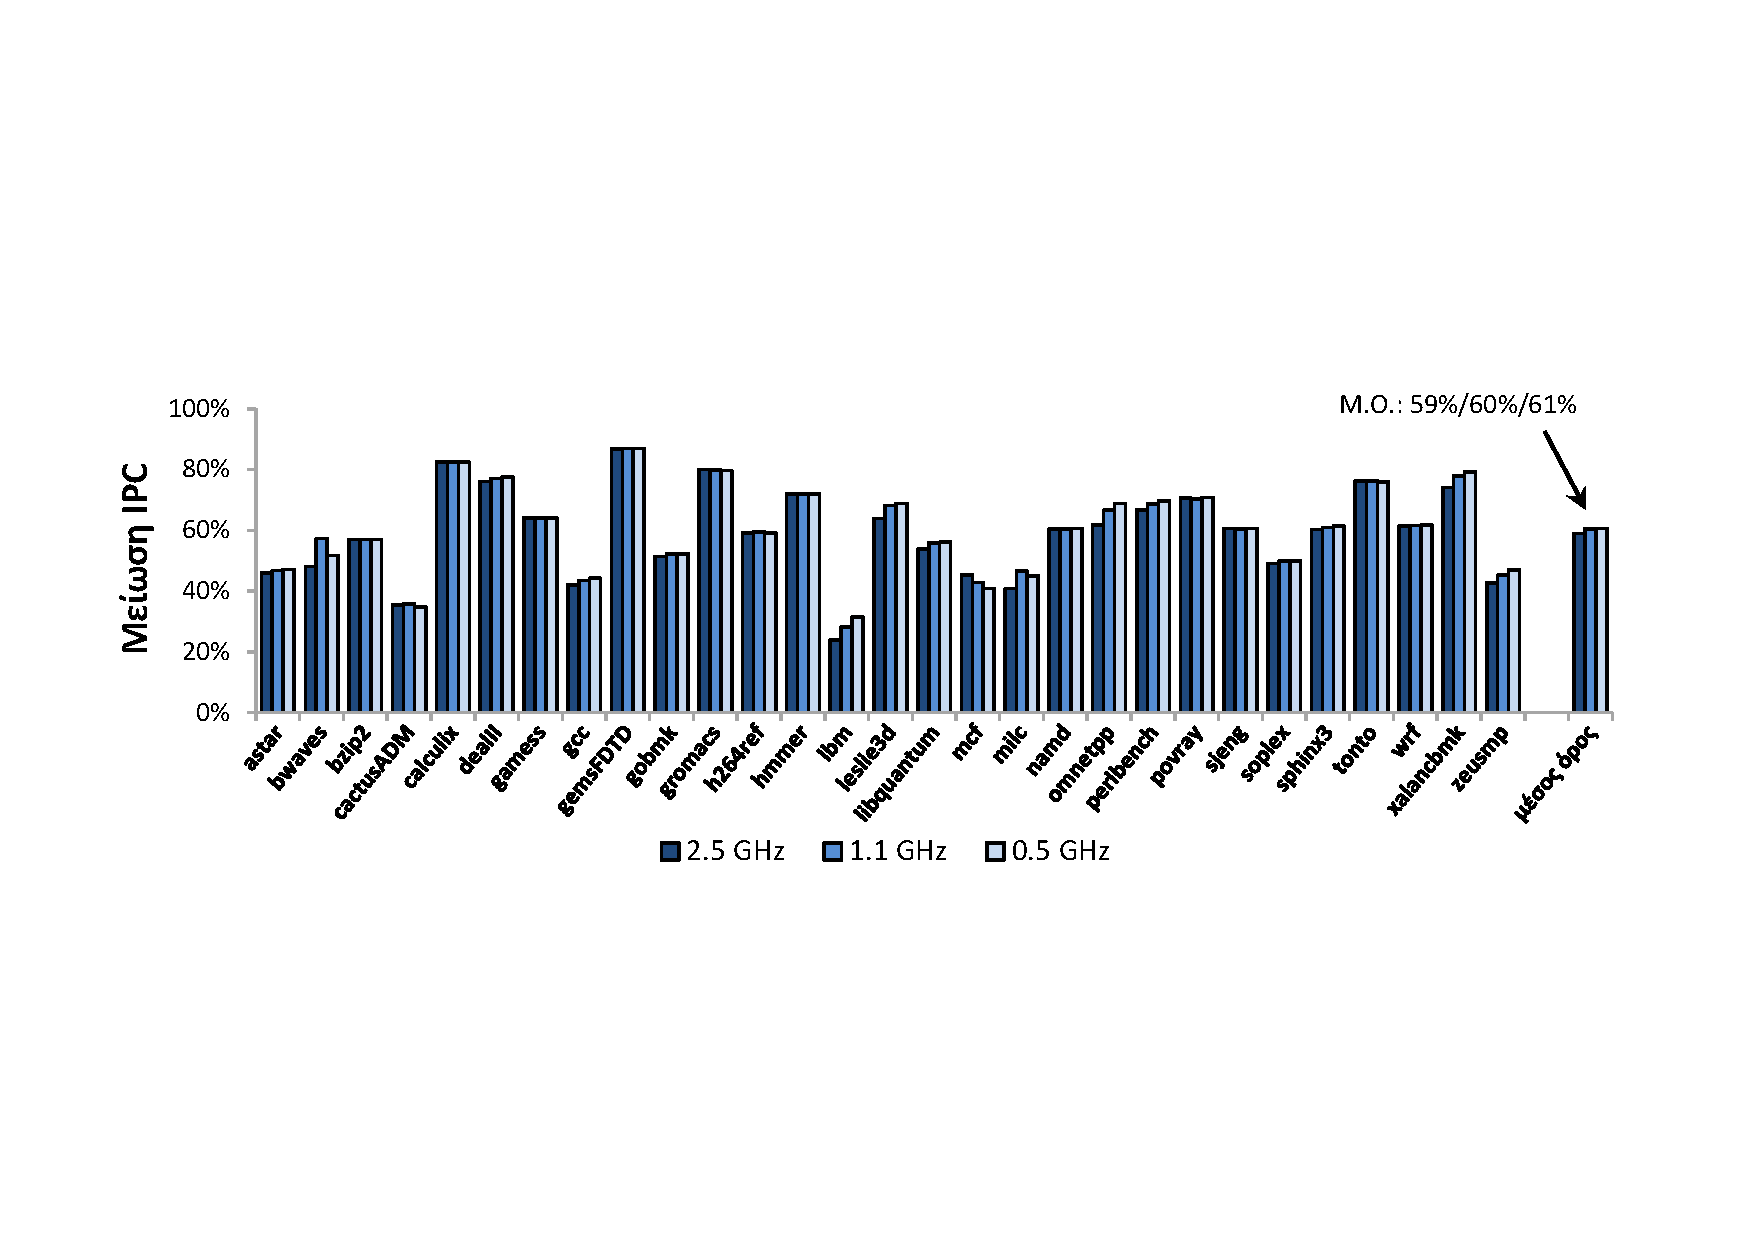
\includegraphics[width=\linewidth, trim=1.9cm 6.4cm 1.8cm 6.6cm, clip=true]{\resultsDIR/chap2_NoPrediction_NoBTB_ipc.pdf}}
    \caption{Ρυθμός ολοκλήρωσης εντολών όταν δεν διατίθεται μηχανισμός πρόβλεψης διακλαδώσεων, κανονικοποιημένος ως προς την περίπτωση που χρησιμοποιείται ο κατάλληλος μηχανισμός}
    \label{fig:chap2_performance_without_prediction}
\end{figure}

Στους σύγχρονους υπερβαθμωτούς επεξεργαστές, η Μονάδα Δυναμικής Πρόβλεψης Διακλαδώσεων \cite{smith1981study} αποτελείται από δύο βασικά στοιχεία. Το πρώτο και σημαντικότερο στοιχείο είναι ο Πίνακας Πρόβλεψης Διακλάδωσης \cite{pan1992improving, quinones2007improving}, η οποία περιέχει την κατάλληλη πληροφορία ώστε να γίνει η πρόβλεψη εάν η εκτέλεση πρέπει να συνεχιστεί στην αμέσως επόμενη εντολή (μη λήψη της διακλάδωσης) ή σε κάποιο άλλο σημείο του προγράμματος (λήψη της διακλάδωσης), δηλαδή εάν θα ικανοποιηθεί η συνθήκη της εντολής διακλάδωσης ή όχι. Το δεύτερο στοιχείο της Μονάδας Δυναμικής Πρόβλεψης Διακλαδώσεων αποτελεί ο Πίνακας Πρόβλεψης Προορισμού Διακλάδωσης \cite{bray1991strategies, perleberg1993branch}. Ο συγκεκριμένος πίνακας αποτελεί μία μνήμη η οποία παρέχει τη διεύθυνση εντολής στην οποία προβλέπεται να μετατοπιστεί η εκτέλεση, σε περίπτωση που έχει προβλεφθεί λήψη της διακλάδωσης από το πρώτο στοιχείο. Η χρήση ενός μηχανισμού πρόβλεψης διακλαδώσεων συνεπάγεται και την ανάγκη για υλοποίηση κατάλληλου μηχανισμού επαναφοράς σε περίπτωση λανθασμένης πρόβλεψης. Η γενική δομή της Μονάδας Δυναμικής Πρόβλεψης Διακλαδώσεων παρουσιάζεται στο Σχήμα \ref{fig:chap2_abstract_predictor}.

\begin{figure}[!b]
    \centering
    \fbox{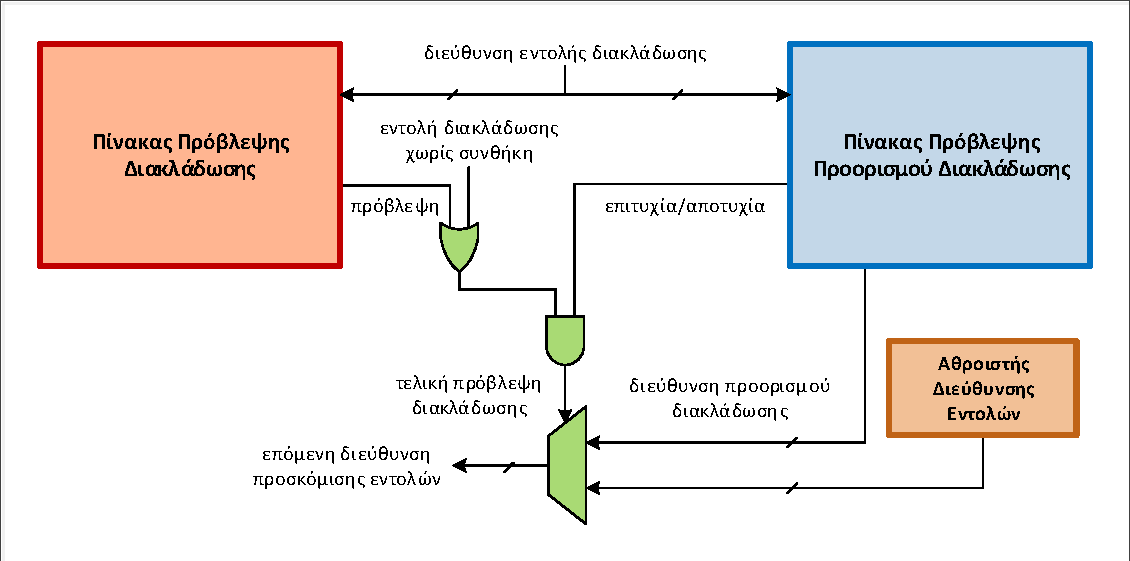
\includegraphics[width=\linewidth, trim=0.5cm 0.65cm 0.5cm 0.7cm, clip=true]{\hardwareDIR/chap2_abstract_predictor.pdf}}
    \caption{Περιληπτική δομή της Μονάδας Δυναμικής Πρόβλεψης Διακλαδώσεων}
    \label{fig:chap2_abstract_predictor}
\end{figure}

%----------------------------------------------------------%

\subsection{Πίνακας Πρόβλεψης Διακλάδωσης}
\label{chap2_BranchPredictor}

Πληθώρα τεχνικών έχουν προταθεί για την υλοποίηση του Πίνακα Πρόβλεψης Διακλάδωσης. Οι τεχνικές αυτές μπορούν να ομαδοποιηθούν σε τρεις κατηγορίες αναλόγως του τρόπου εξαγωγής πρόβλεψης: αυτές που έχουν ως δεδομένο την τρέχουσα τιμή του μετρητή προγράμματος, αυτές που διατηρούν ιστορικό εκτέλεσης των εντολών διακλάδωσης, και τέλος τις συνδυαστικές.
\par
Οι τεχνικές που χρησιμοποιούνται ευρέως στους σύγχρονους επεξεργαστές ανήκουν στην κατηγορία των συνδυαστικών προβλεπτών \cite{cummins2001branch}. Για το λόγο αυτό χρησιμοποιούν ένα ή περισσότερα στοιχεία μνήμης όπου γίνεται η αποθήκευση του ιστορικού διακλαδώσεων ώστε μελλοντικά να μπορεί να πραγματοποιείται μεγαλύτερης ακριβείας πρόβλεψη, με βάση αυτό το ιστορικό. Η τελική πληροφορία που παρέχεται αποτελείται από ένα δυαδικό ψηφίο το οποίο δηλώνει εάν προβλέπεται ότι η μετατόπιση της ροής θα γίνει ή όχι (λήψη/μη λήψη διακλάδωσης). Τον πυρήνα της πρόβλεψης αποτελεί ο αποκαλούμενος Πίνακας Πρόβλεψης Διακλάδωσης ή Πίνακας Ιστορικού Διακλάδωσης, ο οποίος συνήθως αποτελείται από ένα σύνολο μετρητών των δύο δυαδικών ψηφίων. Με τον υπολογισμό του αποτελέσματος της εντολής διακλάδωσης ο αντίστοιχος μετρητής ενημερώνεται κατάλληλα ώστε να γίνει η μετάβαση κατάστασης, όπως φαίνεται και στο διάγραμμα καταστάσεων τους Σχήματος \ref{fig:chap2_2bit_prediction_fsm}.

\begin{figure}[t]
    \centering
    \fbox{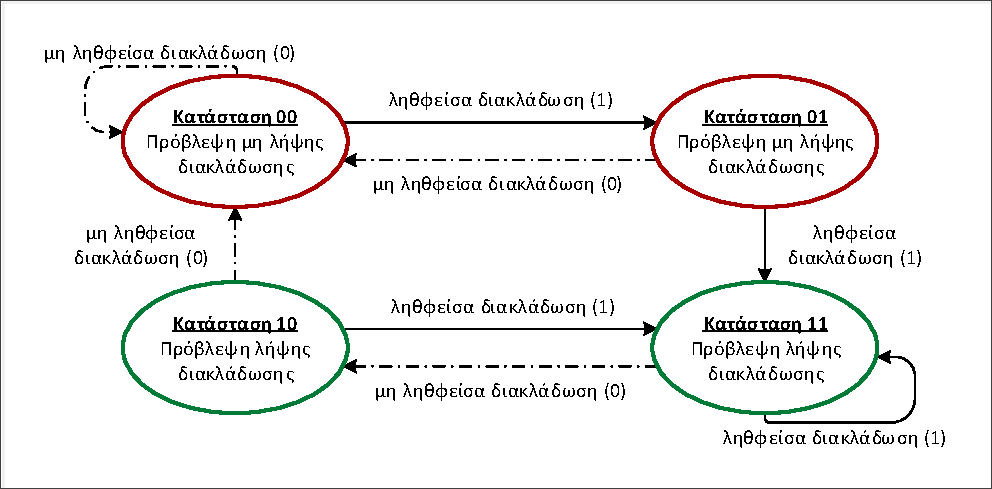
\includegraphics[width=\linewidth, trim=0.3cm 0.7cm 0.3cm 0.7cm, clip=true]{\hardwareDIR/chap2_2bit_prediction_fsm.pdf}}
    \caption{Δυναμική πρόβλεψη δύο δυαδικών ψηφίων}
    \label{fig:chap2_2bit_prediction_fsm}
\end{figure}

Στους μετρητές ιστορικού οι τιμές ‘00’ και ‘01’ αντιστοιχούν σε διατήρηση της ροής εκτέλεσης εντολών (πρόβλεψη μη λήψης διακλάδωσης), σε αντίθεση με τις τιμές ‘10’ και ‘11’ όπου συνεπάγεται πρόβλεψη μετατόπισης της εκτέλεσης (πρόβλεψη λήψης διακλάδωσης). Η ενημέρωση της κατάστασης υλοποιείται μέσω της ολίσθησης των περιεχομένων του αντίστοιχου μετρητή. Επομένως, θεωρώντας πως αρχικά οι μετρητές έχουν τιμή ‘00’, εάν η πρώτη εντολή διακλάδωσης αποδειχθεί πως είναι ληφθείσα (αλλαγή τη ροής) η τιμής του αντίστοιχου μετρητή θα ολισθήσει κατά μία θέση αριστερά και στο λιγότερο σημαντικό ψηφίο θα εισαχθεί το 1 με αποτέλεσμα ο μετρητής να έχει πλέον την τιμή ‘01’. Εάν στην επόμενη εκτέλεση της ίδιας εντολής διακλάδωσης παρουσιαστεί η ίδια συμπεριφορά η τιμή του μετρητή θα γίνει ‘11’. Τη στιγμή που η εντολή αλλάξει τη συμπεριφορά της και η εντολή διακλάδωσης γίνει μη ληφθείσα (η ροή εκτέλεσης παραμένει σταθερή), η τιμή του μετρητή θα ολισθήσει κατά μία θέση αριστερά όπως προηγουμένως, όμως στο λιγότερο σημαντικό ψηφίο θα εισαχθεί το 0. Ώς αποτέλεσμα, η τιμή του μετρητή θα γίνει ‘10’. Αντιστοίχως, την επόμενη φορά που η εντολή διακλάδωσης θα αποδειχθεί μη ληφθείσα ο μετρητής θα πάρει τη τιμή ‘00’.
\par
Στην πραγματικότητα η πρόβλεψη δεν αναφέρεται αποκλειστικά στη συγκεκριμένη εντολή διακλάδωσης αλλά σε ένα πλήθος αυτών, διότι διαφορετικά θα απαιτούνταν στοιχεία μνήμης πολύ μεγάλου μεγέθους για την εξυπηρέτηση όλων των εντολών διακλάδωσης. Η διευθυνσιοδότηση των χρησιμοποιούμενων στοιχείων μνήμης γίνεται είτε από το χαμηλότερο τμήμα της διεύθυνσης των εντολών διακλάδωσης είτε από κάποιο ειδικό καταχωρητή. Το γεγονός αυτό δεν επηρεάζει το αποτέλεσμα της εκτέλεσης. Η μόνη επίπτωση που μπορεί να έχει είναι η μείωση της απόδοσης σε περίπτωση που το ιστορικό έχει αλλοιωθεί εξαιτίας της προσκόμισης και άλλων εντολών διακλάδωσης που επιδρούν στην ίδια θέση μνήμης. Η εξαγωγή μιας λανθασμένης πρόβλεψης θα οδηγήσει στην εκτέλεση λανθασμένου συνόλου εντολών, οι οποίες όμως δεν θα ολοκληρωθούν. Συνεπώς δεν θα αλλοιωθούν τα δεδομένα της κρυφής μνήμης και των καταχωρητών, διότι τα αποτελέσματά των εντολών αναμένουν στη Μονάδα Επαναδιάταξης Αποτελεσμάτων, όπως αναφέρθηκε στην Ενότητα \ref{chap2_Superscalar}. Όταν η εντολή διακλάδωσης εκτελεστεί και αποκαλυφθεί πως έχει ακολουθηθεί λάθος μονοπάτι εντολών, θα εκτελεστεί η διαδικασία απόρριψης εντολών από το Μηχανισμό Μερικώς Επικαλυπτόμενων Λειτουργιών καθώς και η απαραίτητη ενημέρωση της μονάδας πρόβλεψης. Στη συνέχεια γίνεται η προσκόμιση των σωστών εντολών από την Κρυφή Μνήμη Εντολών.

\begin{figure}[!b]
    \centering
    \fbox{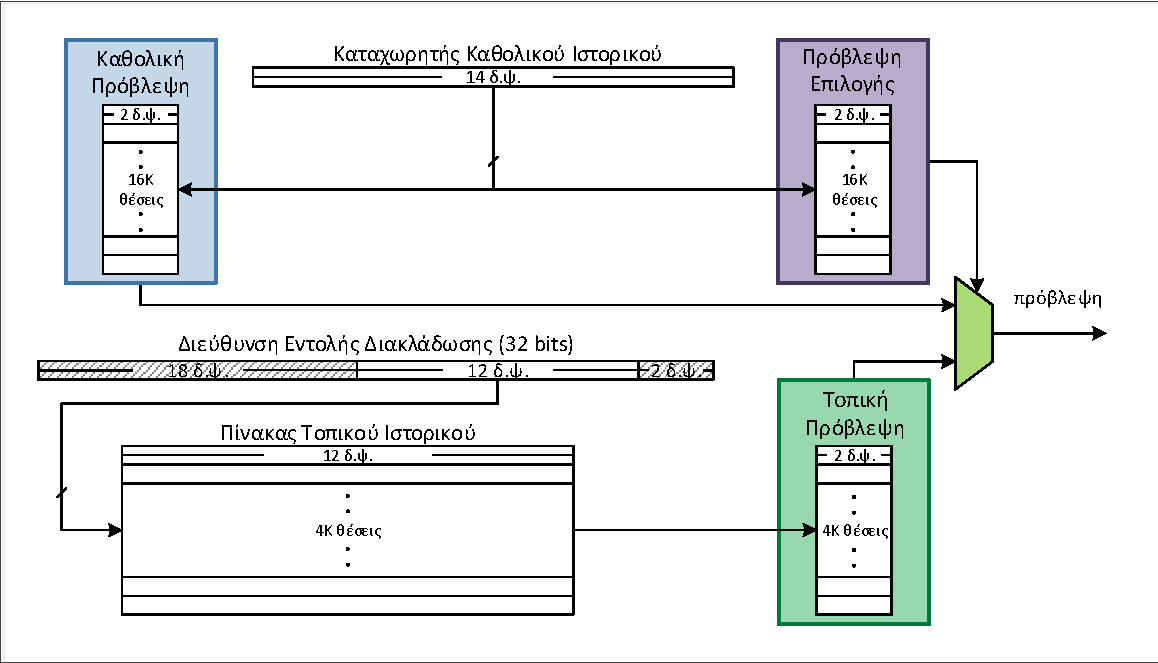
\includegraphics[width=\linewidth, trim=0.45cm 0.6cm 0.45cm 0.6cm, clip=true]{\hardwareDIR/chap2_tournament_predictor.pdf}}
    \caption{Δομή Πρόβλεψης Επιλεκτικής Διάταξης}
    \label{fig:chap2_tournament_predictor}
\end{figure}

Μια από τις πιο διαδεδομένες τεχνικές πρόβλεψης των σύγχρονων υπερβαθμωτών επεξεργαστών είναι η Πρόβλεψη Επιλεκτικής Διάταξης \cite{kessler1998alpha}, η οποία χρησιμοποιεί ένα πλήθος στοιχείων μνήμης ώστε σε κάθε περίπτωση διακλάδωσης να χρησιμοποιηθεί αυτή που έχει μεγαλύτερη πιθανότητα ευστοχίας. Η δομή της τεχνικής αυτής παρουσιάζεται αναλυτικά στο Σχήμα \ref{fig:chap2_tournament_predictor}.
\par
Στην πρόβλεψη επιλεκτικής διάταξης χρησιμοποιούνται δύο διατάξεις εξαγωγής πρόβλεψης διακλάδωσης καθώς και μία διάταξη για την επιλογή της κατάλληλης πρόβλεψης διακλάδωσης. Κάθε στοιχείο πρόβλεψης αποτελείται από ένα πίνακα μετρητών, με κάθε μετρητή να αντιστοιχεί σε ένα σύνολο εντολών. Στην περίπτωση των προβλέψεων διακλάδωσης (Καθολική και Τοπική Πρόβλεψη), το πιο σημαντικό ψηφίο κάθε θέσης του πίνακα μετρητών δηλώνει εάν προβλέπεται να γίνει λήψη ή όχι της διακλάδωσης. Η διάταξη επιλογής (Πρόβλεψη Επιλογής) αποτελείται επίσης από ένα πίνακα μετρητών οπού το πιο σημαντικό ψηφίο κάθε θέσης δηλώνει εάν θα χρησιμοποιηθεί η Καθολική ή η Τοπική Πρόβλεψη. Για τη δεικτοδότηση των μετρητών χρησιμοποιούνται κάποια στοιχεία αποθήκευσης ιστορικού, όπως παρουσιάζεται και στο Σχήμα \ref{fig:chap2_tournament_predictor}.

\subsubsection*{Καταχωρητής Καθολικού Ιστορικού}
\label{chap2_GlobalHistoryBuffer}

Το περιεχόμενό του χρησιμοποιείται για τη διευθυνσιοδότηση τόσο του πίνακα μετρητών της Καθολικής Πρόβλεψης όσο και του αντίστοιχου πίνακα της Πρόβλεψης Επιλογής, επομένως το μέγεθός του εξαρτάται από το πλήθος των μετρητών τους. Κάθε φορά που εξάγεται μία πρόβλεψη από τον Πίνακα Πρόβλεψης Διακλάδωσης, πραγματοποιείται και η ενημέρωση του καταχωρητή. Τα περιεχόμενά του ολισθαίνουν κατά μία θέση προς τα αριστερά και εάν η πρόβλεψη που εξάγεται δηλώνει λήψη της διακλάδωσης το τελευταίο δυαδικό ψηφίο παίρνει την τιμή 1, διαφορετικά την τιμή 0. Σε περίπτωση που η πρόβλεψη αποδειχθεί λανθασμένη, κατά τη διαδικασία απόρριψης των περιττών εντολών γίνεται και η ενημέρωση των περιεχομένων του. Τα περιεχόμενά ολισθαίνουν κατά μία θέση προς τα αριστερά και εάν έγινε λήψη της διακλάδωσης το τελευταίο δυαδικό ψηφίο παίρνει την τιμή 1, διαφορετικά την τιμή 0.

\subsubsection*{Καθολική Πρόβλεψη}
\label{chap2_GlobalPrediction}

Παρέχει μία πρόβλεψη με βάση τη συνολική συμπεριφορά του προγράμματος και όχι της συγκεκριμένης εντολής διακλάδωσης που προσκομίζεται. Αποτελείται από ένα πίνακα μετρητών, συνήθως των δύο δυαδικών ψηφίων. Σε κάθε προσκόμιση εντολής διακλάδωσης το περιεχόμενο του Καταχωρητή Καθολικού Ιστορικού ορίζει ποιο στοιχείο του πίνακα θα παρέχει την πρόβλεψη, η οποία οδηγείται έως τον πολυπλέκτη που ελέγχει η Πρόβλεψη Επιλογής. Όταν υπολογιστεί το αποτέλεσμα της εντολής διακλάδωσης γίνεται η κατάλληλη ενημέρωση του μετρητή που δείχνει ο Καταχωρητής Καθολικού Ιστορικού. Εάν το αποτέλεσμα της εντολής είναι λήψη της διακλάδωσης η τιμή του συγκεκριμένου μετρητή αυξάνεται κατά 1, στην αντίθετη περίπτωση η τιμή του μειώνεται κατά 1. Ο μετρητής που θα ενημερωθεί μπορεί να διαφέρει από αυτόν που χρησιμοποιήθηκε κατά την πρόβλεψη της συγκεκριμένης εντολής διότι μεταξύ της προσκόμισης και της εκτέλεσης της ενδέχεται να έχουν προσκομιστεί και άλλες εντολές διακλάδωσης μεταβάλλοντας έτσι το περιεχόμενο του Καταχωρητή Καθολικού Ιστορικού.

\subsubsection*{Πίνακας Τοπικού Ιστορικού}
\label{chap2_LocalHistoryTable}

Αποτελείται από ένα σύνολο στοιχείων μνήμης πολλαπλών δυαδικών ψηφίων όπου κάθε θέση αντιστοιχεί σε ένα σύνολο εντολών διακλάδωσης, σε αντίθεση με τον Καταχωρητή Καθολικού Ιστορικού ο οποίος αντιστοιχεί σε όλες τις εντολές διακλάδωσης. Η δανειοδοτούμενη θέσης χρησιμοποιείται για τη διευθυνσιοδότηση του πίνακα μετρητών της Τοπικής Πρόβλεψης και ενημερώνεται κατάλληλα όταν εξάγεται μία πρόβλεψη από τον Πίνακα Πρόβλεψης Διακλάδωσης. Σε αντιστοιχία με τον Καταχωρητή Καθολικού Ιστορικού, κάθε φορά που γίνεται μία πρόβλεψη το περιεχόμενο της δεικτοδοτούμενης θέσης του πίνακα ολισθαίνει κατά μία θέση προς τα αριστερά. Όταν προβλέπεται πως θα γίνει λήψη της διακλάδωσης το τελευταίο δυαδικό ψηφίο παίρνει την τιμή 1, διαφορετικά την τιμή 0. Η διευθυνσιοδότηση του πίνακα γίνεται από τα χαμηλότερης τάξης δυαδικά ψηφία της διεύθυνσης της εντολής διακλάδωσης. Κατά τη διαδικασία απόρριψης εντολών σε περίπτωση αποτυχίας πρόβλεψης γίνεται και η ενημέρωση των περιεχομένων της θέσης που δεικτοδοτείται. Η τιμή της ολισθαίνει κατά μία θέση προς τα αριστερά και εάν έγινε λήψη της διακλάδωσης το τελευταίο δυαδικό ψηφίο παίρνει την τιμή 1, διαφορετικά την τιμή 0.

\subsubsection*{Τοπική Πρόβλεψη}
\label{chap2_LocalPrediction}

Παρέχει μία πρόβλεψη με βάση τη συμπεριφορά ενός περιορισμένου συνόλου εντολών διακλάδωσης. Αποτελείται από ένα πίνακα μετρητών, συνήθως των δύο ή τριών δυαδικών ψηφίων για μεγαλύτερη ακρίβεια πρόβλεψης (8 καταστάσεις αντί για 4 στο διάγραμμα καταστάσεων του Σχήματος \ref{fig:chap2_2bit_prediction_fsm}). Όταν γίνεται προσκόμιση μίας εντολής διακλάδωσης μία από τις θέσεις του Πίνακα Τοπικού Ιστορικού καθορίζει ποια θέση του πίνακα θα παρέχει την πρόβλεψη, η οποία οδηγείται στην δεύτερη είσοδο του πολυπλέκτη που ελέγχει η Πρόβλεψη Επιλογής. Όταν υπολογιστεί το αποτέλεσμα της εντολής διακλάδωσης γίνεται και η κατάλληλη ενημέρωση του δεικτοδοτούμενου μετρητή. Εάν το αποτέλεσμα της εντολής είναι λήψη της διακλάδωσης η τιμή του συγκεκριμένου μετρητή αυξάνεται κατά 1, στην αντίθετη περίπτωση η τιμή του μειώνεται κατά 1. Ομοίως με την περίπτωση της Καθολικής Πρόβλεψης, ο μετρητής που θα ενημερωθεί μπορεί να διαφέρει από αυτόν που χρησιμοποιήθηκε κατά την πρόβλεψη της συγκεκριμένης εντολής, εξαιτίας της μεταβολής των περιεχομένων του Πίνακα Τοπικού Ιστορικού.

\subsubsection*{Πρόβλεψη Επιλογής}
\label{chap2_ChoicePrediction}

Παρέχει την πρόβλεψη για τη σωστή επιλογή μεταξύ της Τοπικής και της Καθολικής Πρόβλεψης, με βάση τη συνολική συμπεριφορά του προγράμματος. Αποτελείται από ένα πίνακα μετρητών, συνήθως των δύο δυαδικών ψηφίων και μεγέθους όσο και ο αντίστοιχος πίνακας της Καθολικής Πρόβλεψης. Το περιεχόμενο του Καταχωρητή Καθολικού Ιστορικού ορίζει ποια θέση του πίνακα θα παρέχει την πρόβλεψη επιλογής, και το πιο σημαντικό ψηφίο αυτής της θέσης οδηγείται στην είσοδο ελέγχου του πολυπλέκτη. Όταν υπολογιστεί το αποτέλεσμα της εντολής διακλάδωσης γίνεται η κατάλληλη ενημέρωση του μετρητή που δείχνει ο Καταχωρητής Καθολικού Ιστορικού, εάν και μόνο εάν οι προβλέψεις των δύο διατάξεων (Καθολική/Τοπική) διαφέρουν μεταξύ τους. Εάν το αποτέλεσμα της διακλάδωσης συμπίπτει με την Τοπική Πρόβλεψη η τιμή του συγκεκριμένου μετρητή μειώνεται κατά 1, διαφορετικά αυξάνεται κατά 1. Όπως με την περίπτωση της Καθολικής Πρόβλεψης, ο μετρητής που θα ενημερωθεί μπορεί να διαφέρει από αυτόν που χρησιμοποιήθηκε κατά την πρόβλεψη της εντολής.

\subsubsection*{Διάγραμμα Ενημέρωσης Στοιχείων Πρόβλεψης}
\label{chap2_PredictionUpdate}

Στο Σχήμα \ref{fig:chap2_predictor_update} παρουσιάζονται διαγραμματικά οι συνθήκες που ισχύουν για την ενημέρωση των στοιχείων μνήμης που αποτελούν τον Πίνακα Πρόβλεψης Διακλάδωσης. Oι συμβολισμοί $``\ +$1 $"$, $``\ -$1 $"$, $``\ <<1\ "$ και $``\ <<1$ \& +1 $"$ ισοδυναμούν με αύξηση κατά μία μονάδα, μείωση κατά μία μονάδα, αριστερή ολίσθηση κατά ένα δυαδικό ψηφίο, αριστερή ολίσθηση κατά ένα δυαδικό ψηφίο και εισαγωγή της μονάδας στο λιγότερο σημαντικό ψηφίο αντίστοιχα.

\begin{figure}[!h]
    \centering
    \fbox{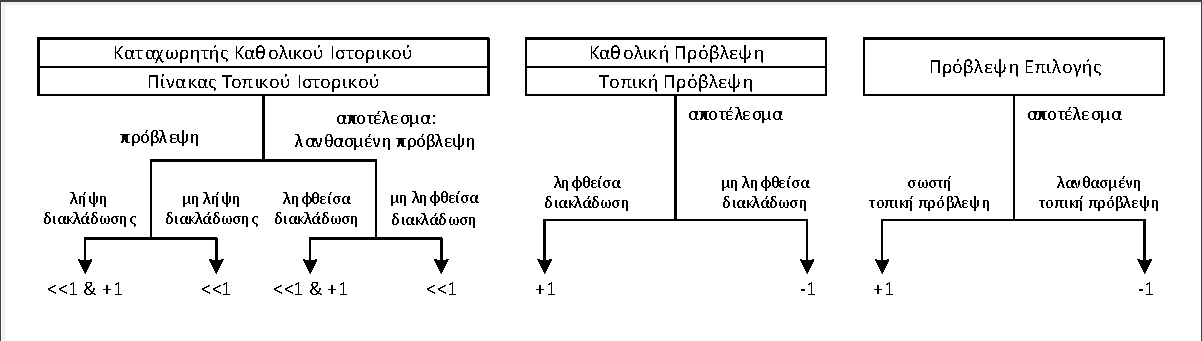
\includegraphics[width=\linewidth, trim=0.5cm 0.8cm 0.5cm 0.6cm, clip=true]{\hardwareDIR/chap2_predictors_update.pdf}}
    \caption{Μεθοδολογία ενημέρωσης των στοιχείων που συμβάλουν στην πρόβλεψη}
    \label{fig:chap2_predictor_update}
\end{figure}

%----------------------------------------------------------%

\subsection{Πίνακας Πρόβλεψης Προορισμού Διακλάδωσης}
\label{chap2_BranchTargetBuffer}

Σε μία σύγχρονη αρχιτεκτονική περικλείονται πολλών ειδών εντολές διακλάδωσης, οι οποίες παρουσιάζουν σημαντικές διαφορές στη συμπεριφορά τους και για το λόγο αυτό κατηγοριοποιούνται. Συνεπώς, προτού γίνει εμβάθυνση στη λειτουργία της συγκεκριμένης μνήμης είναι απαραίτητο να αποσαφηνιστούν οι διαφορές μεταξύ τους. Στην ακόλουθη περιγραφή των κατηγοριών, για κάθε κατηγορίας εντολής διακλάδωσης δίνεται και ένα παράδειγμα από το σύνολο εντολών αρχιτεκτονικής \en{MIPS} \cite{price1995mips}.
\par
Οι εντολές διακλάδωσης που προσκομίζονται στο Μηχανισμό Μερικώς Επικαλυπτόμενων Λειτουργιών διαχωρίζονται στις ακόλουθες δύο κατηγορίες:\\
\indent\textbf{\textit{Άμεσης Διευθυνσιοδότησης -}} Η διεύθυνση στην οποία θα μεταβεί η εκτέλεση σε περίπτωση που γίνει λήψη της διακλάδωσης αποτελεί τμήμα της εντολής και είναι ήδη γνωστή. Παράδειγμα τέτοιου είδους εντολής διακλάδωσης αποτελεί η εντολή \en{J} ενός επεξεργαστή \en{MIPS}.\\
\indent\textbf{\textit{Έμμεσης Διευθυνσιοδότησης -}} Η διεύθυνση στην οποία θα μεταβεί η εκτέλεση σε περίπτωση που γίνει λήψη της διακλάδωσης δεν είναι γνωστή εκ των προτέρων, ως εκ τούτου απαιτείται επιπλέον χρόνο για τον υπολογισμό της. Ο Πίνακας Πρόβλεψης Προορισμού Διακλάδωσης διατηρεί ένα ιστορικό των διευθύνσεων διακλάδωσης με βάση την προηγούμενη συμπεριφορά των εντολών, ώστε να παρέχει μία πρόβλεψης της διεύθυνσης στην οποία θα μεταφερθεί η εκτέλεση του προγράμματος προτού γίνει ο πραγματικός υπολογισμός της για την επαλήθευση της πρόβλεψης. Παράδειγμα τέτοιου είδους εντολής διακλάδωσης στον \en{MIPS} αποτελεί η εντολή \en{JR}.
\par
Επιπλέον, οι εντολές διακλάδωσης (άμεσης και έμμεσης διευθυνσιοδότησης) μπορούν να διαχωριστούν στις ακόλουθες δύο υποκατηγορίες:\\
\indent\textbf{\textit{Χωρίς Συνθήκη -}} Η συμπεριφορά της εντολής διακλάδωσης είναι προκαθορισμένη και επομένως το μόνο που απαιτείται είναι μία πρόβλεψη της διεύθυνσης στην οποία θα γίνει η μετατόπιση της εκτέλεσης. Όταν η εντολή είναι έμμεσης διευθυνσιοδότηση η πληροφορία αυτή λαμβάνεται από τον Πίνακα Πρόβλεψης Προορισμού Διακλάδωσης, εάν είναι διαθέσιμη. Παράδειγμα τέτοιου είδους εντολής διακλάδωσης στον \en{MIPS} αποτελεί η εντολή \en{JR}.\\
\indent\textbf{\textit{Υπό Συνθήκη -}} Ο Πίνακας Πρόβλεψης Διακλάδωσης παρέχει την πρόβλεψη εάν θα γίνει λήψη της διακλάδωση καθώς δεν είναι γνωστή εκ των προτέρων η συμπεριφορά των εντολών αυτού του είδους. Σε περίπτωση που προβλέπεται λήψη της διακλάδωσης και η εντολή είναι έμμεσης διευθυνσιοδότηση, ο Πίνακας Πρόβλεψης Προορισμού Διακλάδωσης παρέχει μία πρόβλεψη της διεύθυνσης μετατόπισης της ροής εκτέλεσης, εάν έχει διαθέσιμη την πληροφορία αυτή. Παράδειγμα τέτοιου είδους εντολής διακλάδωσης στον \en{MIPS} αποτελεί η εντολή \en{BEQ}.
\par
Επομένως, στην περίπτωση των εντολών έμμεσης διευθυνσιοδότησης η γνώση - πρόβλεψη της διεύθυνσης στην οποία θα μεταφερθεί η εκτέλεση αποτελεί σημαντικό πλεονέκτημα για την επικάλυψη του χρόνου καθυστέρησης που εισάγεται έως τον υπολογισμό της.

\begin{figure}[!b]
    \centering
    \fbox{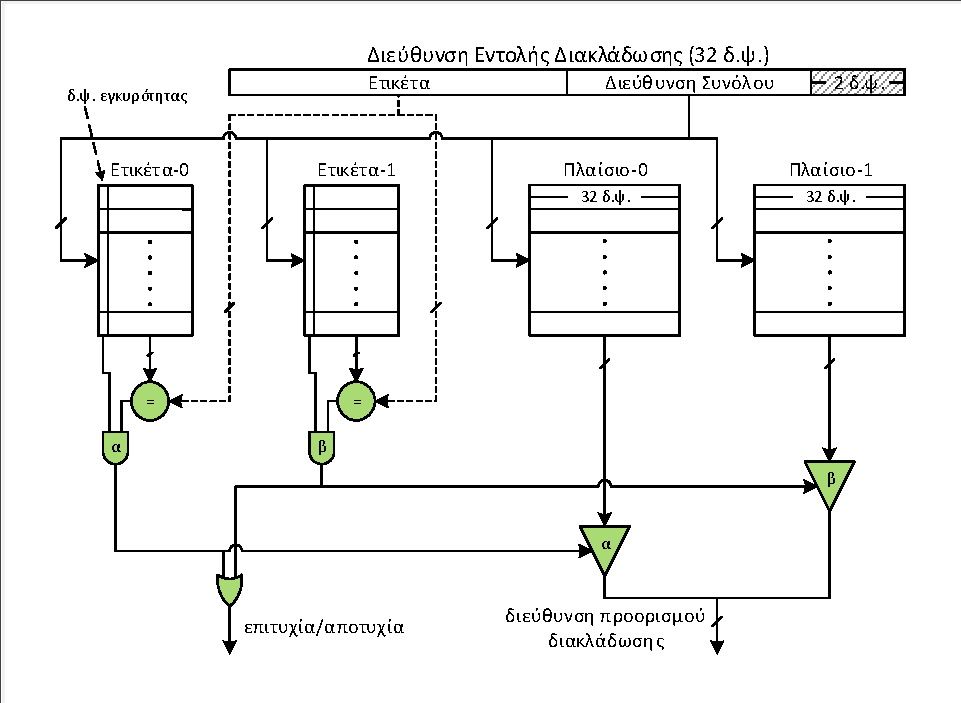
\includegraphics[width=\linewidth, trim=0.5cm 0.8cm 0.5cm 0.7cm, clip=true]{\hardwareDIR/chap2_btb.pdf}}
    \caption{Δομή Πίνακα Πρόβλεψης Προορισμού Διακλάδωσης}
    \label{fig:chap2_branch_target_buffer}
\end{figure}

\par
Ο Πίνακας Πρόβλεψης Προορισμού Διακλάδωσης αποτελεί ένα στοιχείο μνήμης αντίστοιχο μίας Κρυφής Μνήμης οργάνωσης τ-τρόπως συνόλου συσχέτισης \cite{nikolos2012architecture}. Διαχωρίζεται δηλαδή σε σύνολα με το καθένα να αποτελείται από τ πλαίσια μνήμης. Κάθε διεύθυνση μνήμης αντιστοιχίζεται σε ένα σύνολο και η διευθυνσιοδότηση της (δεικτοδότηση συνόλου) γίνεται από τα χαμηλότερης τάξης δυαδικά ψηφία της διεύθυνσης της εντολής διακλάδωσης, όπως παρουσιάζεται και στο Σχήμα \ref{fig:chap2_branch_target_buffer}. Με τον τρόπο αυτό σε ένα σύνολο μπορούν να βρίσκονται αποθηκευμένες πολλαπλές πληροφορίες παράλληλα, με κάθε πληροφορία να καταλαμβάνει μία θέση διεύθυνσης προορισμού καθώς και το αντίστοιχο πεδίο ετικέτας. Επομένως, ένα πλήθος εντολών διακλάδωσης θα αντιστοιχίζεται στο ίδιο σύνολο του Πίνακα Πρόβλεψης Προορισμού Διακλάδωσης.
\par
Όταν μια εντολή διακλάδωσης προσκομιστεί, ταυτόχρονα με την πρόβλεψη λήψης της διακλάδωσης γίνεται και η προσπέλαση του Πίνακα Πρόβλεψης Προορισμού Διακλάδωσης. Όπως και στην περίπτωση των κρυφών μνημών πρώτου επιπέδου, χρησιμοποιώντας το πεδίο ετικέτας της διεύθυνσης εντολής καθώς και τα κατάλληλα ψηφία διευθυνσιοδότηση, γίνεται αναζήτηση της πληροφορίας στο σύνολο που δεικτοδοτείται. Όταν το πεδίο ετικέτας της εντολής ταυτίζεται με την αποθηκευμένη ετικέτα σε κάποιο από τα στοιχεία του συνόλου και το αντίστοιχο ψηφίο εγκυρότητας είναι ενεργό (1), συνεπάγεται επιτυχία της μνήμης. Η αποθηκευμένη πληροφορία της θέσης διεύθυνσης προορισμού αποστέλλεται ως επόμενη διεύθυνση προσκόμισης εντολής εάν και μόνο εάν ο Πίνακας Πρόβλεψης Διακλάδωσης έχει αποφανθεί λήψη της διακλάδωσης. Στην αντίθετη περίπτωση, όπου είτε η ετικέτα δεν επαληθεύεται είτε το ψηφίο εγκυρότητας είναι μη ενεργό (0), συνεπάγεται πως έχουμε αποτυχία της μνήμης και συνηθισμένη τακτική είναι η αλλαγή της πρόβλεψης σε μη λήψη της διακλάδωσης.
\par
Σε περίπτωση που ο Πίνακας Πρόβλεψης Διακλάδωσης έχει εξάγει πρόβλεψη λήψης της διακλάδωσης, αποτέλεσμα της αποτυχίας του Πίνακα Πρόβλεψης Προορισμού Διακλάδωσης θα είναι η μετατροπή της πρόβλεψης σε μη λήψη της, με μία από τις δύο ακόλουθες συνέπειες:\\
\indent\textit{\textbf{Αρχική πρόβλεψη σωστή:}} Εξαιτίας της λανθασμένης διατήρησης της ροής προσκόμισης εντολών, λανθασμένες εντολές θα προσκομιστούν στην κεντρική μονάδα επεξεργασίας οι οποίες δεν θα ολοκληρωθούν. Όταν υπολογιστεί η εντολή διακλάδωσης, το λάθος της πρόβλεψης θα ανιχνευθεί και οι εντολές που επακολούθησαν θα απορριφθούν από το Μηχανισμό Μερικώς Επικαλυπτόμενων Λειτουργιών. Σε αυτή την περίπτωση συνεπάγεται μείωση της απόδοσης εξαιτίας της αποτυχίας στον Πίνακα Πρόβλεψης Προορισμού Διακλάδωσης.\\
\indent\textit{\textbf{Αρχική πρόβλεψη λανθασμένη:}} Παρότι η αρχική πρόβλεψη θα αποδεικνυόταν μελλοντικά λανθασμένη, η αποτυχία του Πίνακα Πρόβλεψης Προορισμού Διακλάδωσης θα οδηγήσει σε μεταβολή της πρόβλεψης από λανθασμένη σε σωστή. Έτσι θα προσκομιστούν οι σωστές εντολές και συνεπώς θα υπάρξει βελτίωση της απόδοσης εξαιτίας της αποτυχίας στον Πίνακα Πρόβλεψης Προορισμού Διακλάδωσης. Το γεγονός αυτό παρατηρήθηκε και στις εξομοιώσεις που εκτελέστηκαν. Σε ορισμένες περιπτώσεις ενώ το πλήθος των αποτυχιών στον Πίνακα Πρόβλεψης Προορισμού Διακλάδωσης αυξάνεται ο συνολικός χρόνος εκτέλεσης του προγράμματος μειώνεται.

\begin{figure}[t]
    \centering
    \fbox{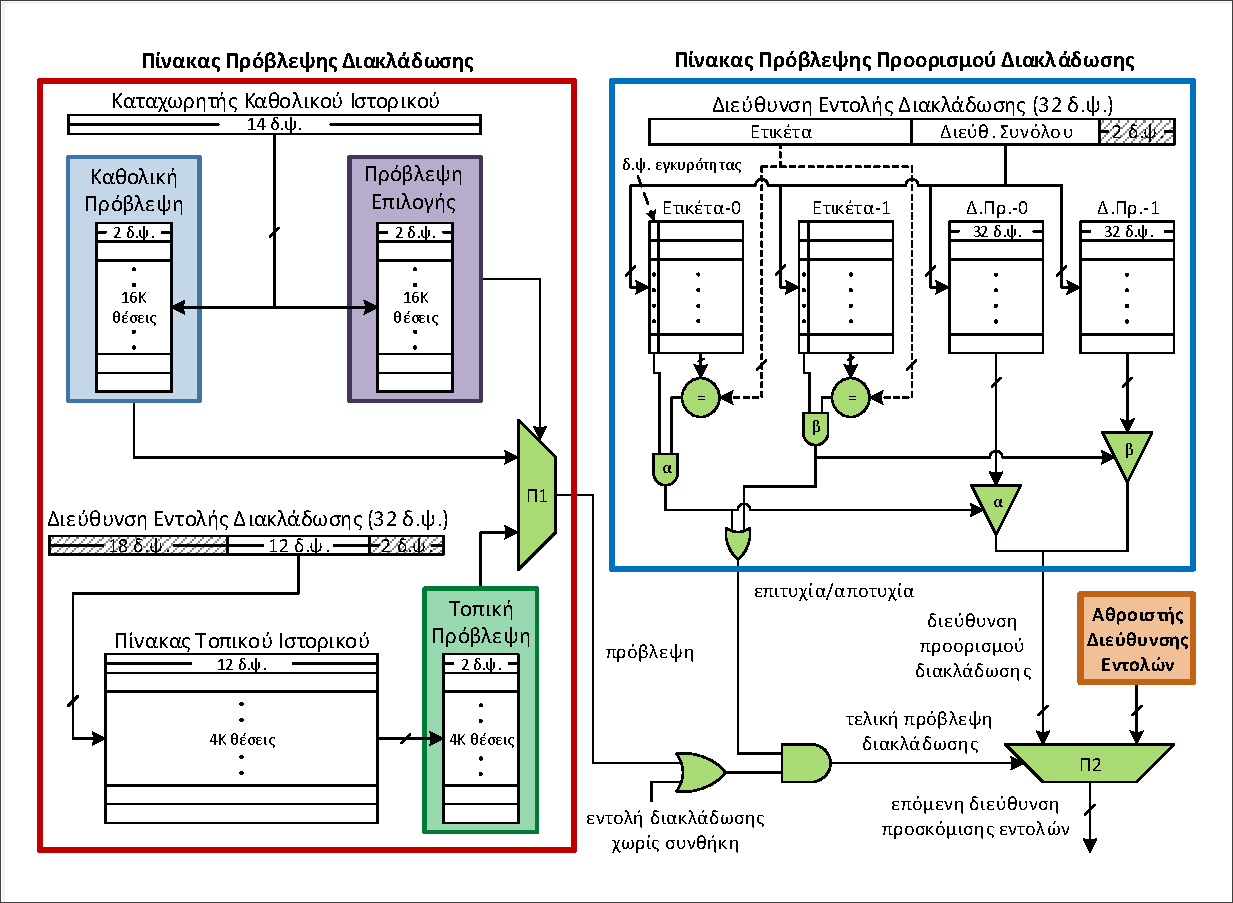
\includegraphics[width=\linewidth, trim=0.5cm 0.8cm 0.5cm 0.8cm, clip=true]{\hardwareDIR/chap2_dynamic_predictor.pdf}}
    \caption{Συνολική δομή της Μονάδας Δυναμικής Πρόβλεψης Διακλαδώσεων}
    \label{fig:chap2_dynamic_predictor}
\end{figure}

Μόλις η εντολή διακλάδωσης εκτελεστεί και αποφανθεί εάν η πρόβλεψη ήταν σωστή ή όχι, γίνεται η κατάλληλη ενημέρωση της αντίστοιχης θέσης του Πίνακα Πρόβλεψης Προορισμού Διακλάδωσης ώστε να ενημερωθεί το πεδίο της διεύθυνσης στην οποία έγινε η μετατόπιση της εκτέλεσης του προγράμματος. Με τον τρόπο αυτό αυξάνεται η λόγος επιτυχίας του την επόμενη φορά που θα προσκομιστεί η ίδια εντολή διακλάδωσης. Ομοίως με τις Κρυφές Μνήμες πρώτου επιπέδου, εξαιτίας του περιορισμένου αριθμού πλαισίων ανά σύνολο απαιτείται η χρήση μίας μεθόδου αντικατάστασης ώστε όταν δεν υπάρχουν διαθέσιμα πλαίσια για την αποθήκευση της κατάλληλης πληροφορίας μίας νέας εντολής διακλάδωσης να πραγματοποιείται αντικατάσταση των δεδομένων μίας δεσμευμένης θέσης. Συνηθισμένη μέθοδος αντικατάστασης είναι αυτή του Λιγότερο Πρόσφατα Χρησιμοποιηθέντος (\en{LRU}) στοιχείου \cite{sudarshan2004highly, al2004performance}, η οποία έχει αποδειχθεί εύκολα υλοποιήσιμη και αρκετά αποδοτική.
\par
Στο Σχήμα \ref{fig:chap2_dynamic_predictor} παρουσιάζεται η συνολική δομή της Μονάδας Δυναμικής Πρόβλεψης Διακλαδώσεων, όπου τα αποτελέσματα των δύο πινάκων οδηγούνται σε κατάλληλες πύλες ώστε να αποφανθεί η διεύθυνση κρυφής μνήμης εντολών από την οποία θα προσκομιστούν οι επόμενες εντολές.

%----------------------------------------------------------%

\subsection{Δειγματοληπτικά Στοιχεία Εντολών Διακλάδωσης}

Η μελέτη της αποδοτικής εξαγωγής προβλέψεων απασχολεί τους ερευνητές από τα πρώτα στάδια ανάπτυξης του υπερβαθμωτού επεξεργαστή. Πολλές μελέτες έχουν επικεντρωθεί στην ανάλυση τους όπως για παράδειγμα τα \cite{Lee2003ExploitingCT} και \cite{eyerman2006characterizing}. Όπως είναι αναμενόμενο, τα μετροπρογράμματα παρουσιάζουν διαφορές στη συμπεριφορά τους. Ορισμένα από αυτά αποτελούνται από αρκετές εντολές διακλάδωσης και επομένως η επιτυχία της Μονάδας Δυναμικής Πρόβλεψης Διακλαδώσεων συμβάλει σημαντικά στην ταχύτερη εκτέλεσή τους.
\par
Το ποσοστό πλήθους και είδους εντολών διακλάδωσης παρουσιάζονται στο Σχήμα \ref{fig:chap2_branch_instr_stats} όπου το άθροισμα των πορτοκαλί και μπλε αποχρώσεων δηλώνει το ποσοστό των εντολών διακλάδωσης σε σχέση με τις συνολικές εντολές που προσκομίζονται, για κάθε μετροπρόγραμμα \spec ξεχωριστά. Οι πορτοκαλί αποχρώσεις αποτελούν ένα τμήμα του συνόλου των εντολών διακλάδωσης και δηλώνουν το ποσοστό αυτών που χρησιμοποιούν τον Πίνακα Πρόβλεψης Προορισμού Διακλάδωσης (ΠΠΠΔ).
\par
Η γραφική παράσταση φανερώνει τις περιπτώσεις μετροπρογραμμάτων οι οποίες θα εκμεταλλευτούν κατά το μέγιστο τον Πίνακα Πρόβλεψης Προορισμού Διακλάδωσης, ο οποίος μελετάται στην παρούσα διπλωματική, και επομένως ο χρόνος εκτέλεσής τους θα εξαρτάται ιδιαίτερα από την ευστοχία του.

\begin{figure}[!h]
    \centering
    \fbox{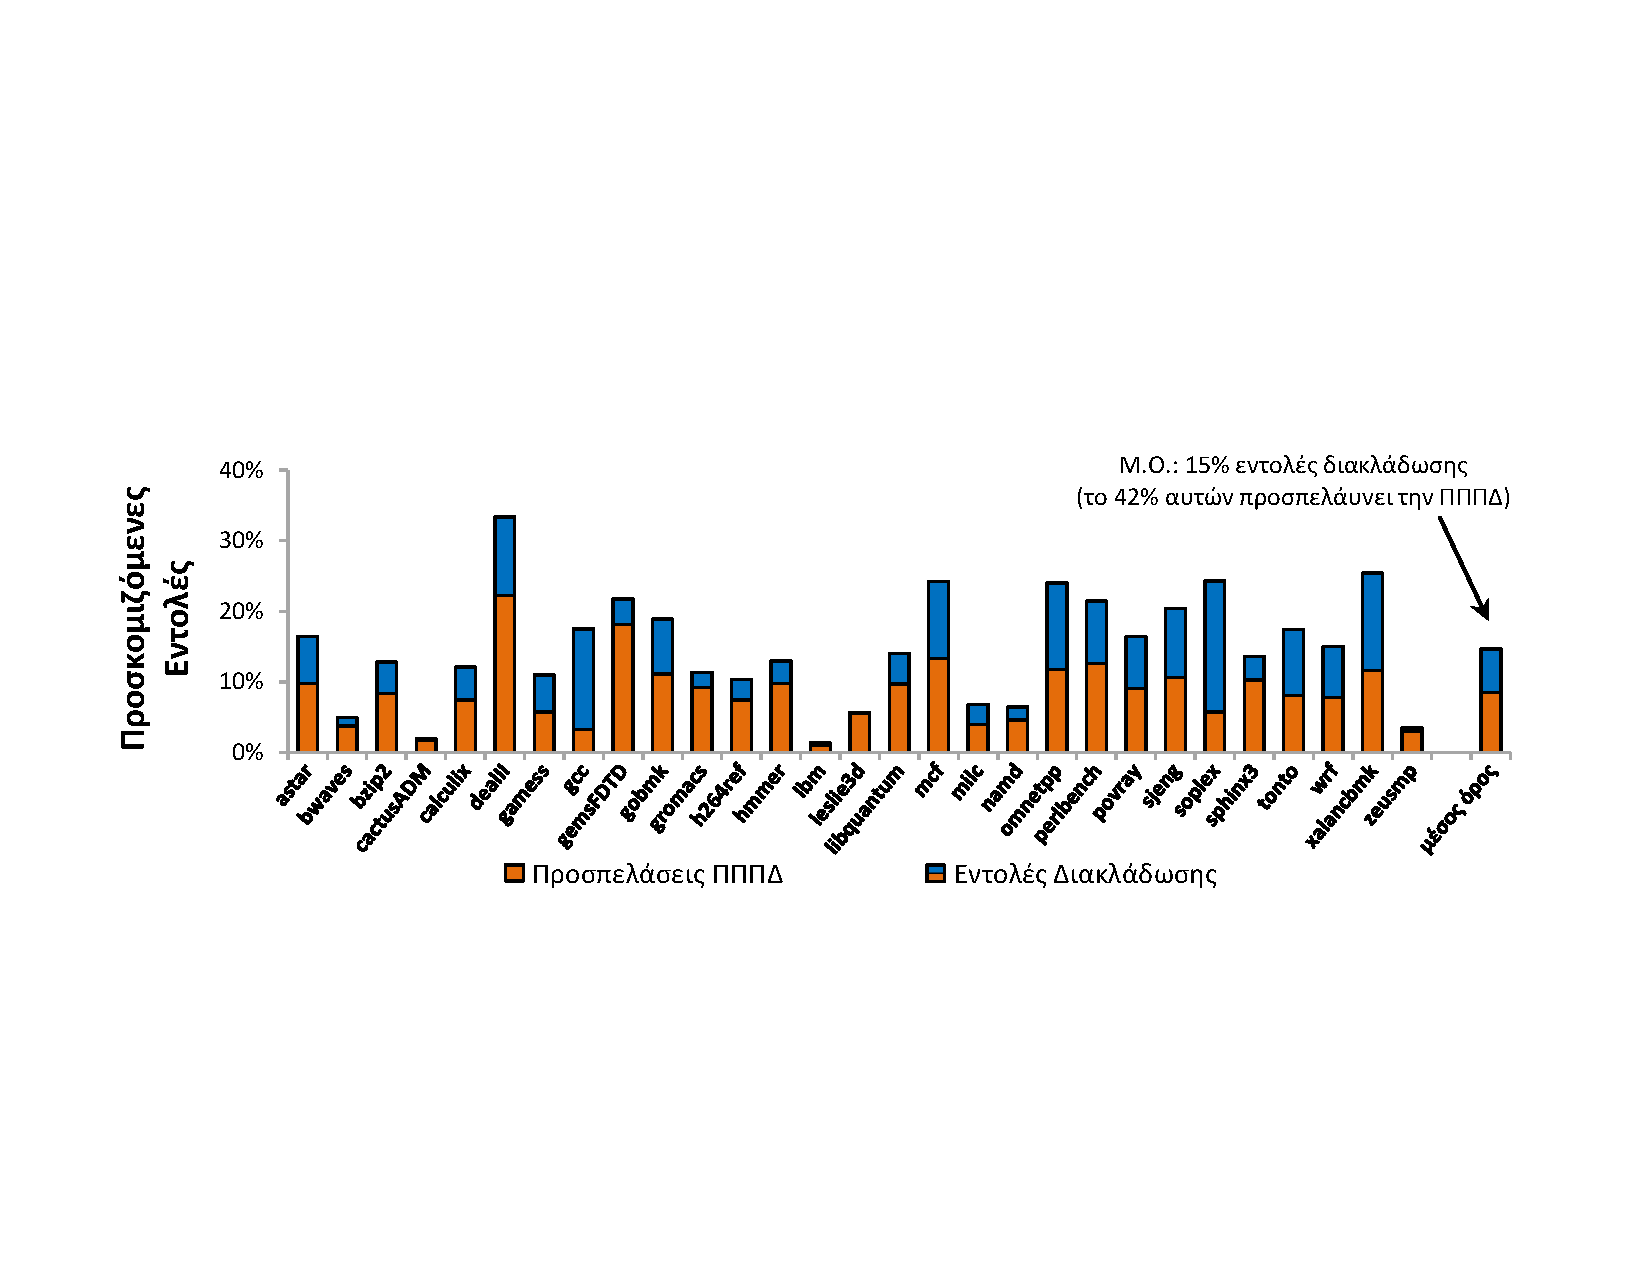
\includegraphics[width=\linewidth, trim=1.9cm 6.5cm 1.8cm 6.6cm, clip=true]{\resultsDIR/chap2_branch_insts.pdf}}
    \caption{Ποσοστό εντολών διακλάδωσης ως προς το σύνολο των προσκομισθέντων εντολών και ποσοστό εντολών διακλάδωσης που προσπελαύνουν τον Πίνακα Πρόβλεψης Προορισμού Διακλάδωσης}
    \label{fig:chap2_branch_instr_stats}
\end{figure}

%----------------------------------------------------------%
